\Chapter{La fusion par confinement magnétique}
\label{AnnexeA}
\begin{refsection}

\section*{La fusion et les tokamaks}

La fusion thermonucléaire, qui a naturellement lieu dans le coeur des étoiles,
est un processus où deux noyaux atomiques s'assemblent pour former un noyau
plus lourd en dégageant une énergie proportionnelle à la perte de masse suivant
l'équation d'Einstein $E=mc^2$. C'est la source d'énergie la plus prometteuse
à ce jour pour soutenir le besoin croissant en énergie de notre civilisation,
économiquement pérenne, techniquement faisable et écologiquement durable.
Au vu de l'énergie libérée et des sections efficaces de réactions envisageables
entre noyaux, la réaction la plus propice à la production d'énergie est la
fusion deutérieum-tritium (D--T), deux isotopes de l'hydrogène, qui produit une
particule $\alpha$ (une particule d'hélium) et un neutron :
\begin{figure}[!htbp]
    \centering
	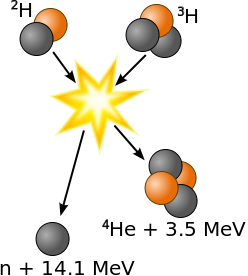
\includegraphics[height=60mm]{figures/1-fusion.png}
	\caption{Réaction
de fusion entre le deutérium et tritium suivant l'équation
bilan : $\ce{^2\text{H}}+\ce{^3\text{H}} \rightarrow
\ce{^4\text{H}}\;(3.5\,\text{MeV})+\text{n}\;(14\,\text{MeV})$}\label{fusionDT}
\end{figure}

Cette réaction ne peut se produire que si l'énergie cinétique des particules
dépasse la répulsion mutuelle des noyaux de charge positive (i.e. à des
température de l'ordre de 10 keV à 100 keV, soit plusieurs centaines de
millions de degrés Celcius). L'agitation thermique ayant de plus tendance à
disperser le plasma, celui-ci doit être confiné (i.e. maintenu dans un volume
fini) par des forces extérieures pour atteindre un équilibre favorable à la
réalisation de réactions de fusion.

Afin que la fusion puisse être énergétiquement rentable, il est nécessaire
que l’énergie produite soit supérieure à la somme de l’énergie perdue hors du
système et de celle consommée par les réactions. Cette contrainte, connue sous
le nom de critère de Lawson~\parencite{Lawson}, s'exprime sous la forme
$nT_i\tau_E>f(Q)$ où $n$ est la densité du plasma, $T_i$ la température ionique
et $\tau_E$ un temps caractéristique de relaxation de l'énergie en l'absence de
toute source de chauffage qui mesure la qualité de confinement du plasma. Le
facteur d'amplification $Q$ représente le ratio entre la puissance dégagée par
les réactions de fusion et celle injectée dans le plasma. L'obtention d'un
facteur d'amplification $Q\geq$40 implique par exemple $nT_i\tau_E\geq$~2.7
10$^{21}$~m$^{-3}$.keV.s$^{-1}$.

Deux voies de recherche sont actuellement explorées
pour reproduire la fusion de manière contrôlée :

\begin{itemize}
	\item La fusion par confinement inertiel chauffe compresse des petites
	billes de D--T par des faisceaux lasers intenses pour obtenir un plasma
	extrêmement dense ($n\sim$10$^{31}$~m$^{-3}$) avec un temps de confinement
	d'énergie très court ($\tau_E\sim$10$^{-11}$~s). Les plus grandes
	expérimentations sont le National Ignition Facility (NIF) aux États-Unis et le
	Laser Mégajoule en France.
	\item La fusion par confinement magnétique est au contraire dans l'optique de
	confiner un plasma de densité plus modeste ($n\sim$10$^{20}$~m$^{-3}$) sur des
	temps bien plus longs ($\tau_E\sim$1~s), à l'aide d'un champ magnétique
	intense. Le projet ITER (International Thermonuclear
	Experimental Reactor~\parencite{ITER}), qui est un projet de coopération
	internationale, a pour objectif de construire le premier prototype de
	réacteur à fusion de type tokamak~\parencite{Wesson}, avec un facteur d'amplification
	$Q\geq$10.
\end{itemize}

Le principe des tokamaks fut inventé au début des années 1950 par les Russes Igor Tamm et
Andreï Sakharov. Les tokamaks sont des machines qui utilisent
un champ magnétique de plusieurs Teslas (13T pour ITER) dont les lignes de
champs s'enroulent hélicoïdalement et se referment sur elles-mêmes de façon à ce que le plasma soit
confiné dans un volume fini (cf. figure~\ref{tokamak}).
\begin{figure}[!htbp]
    \centering
	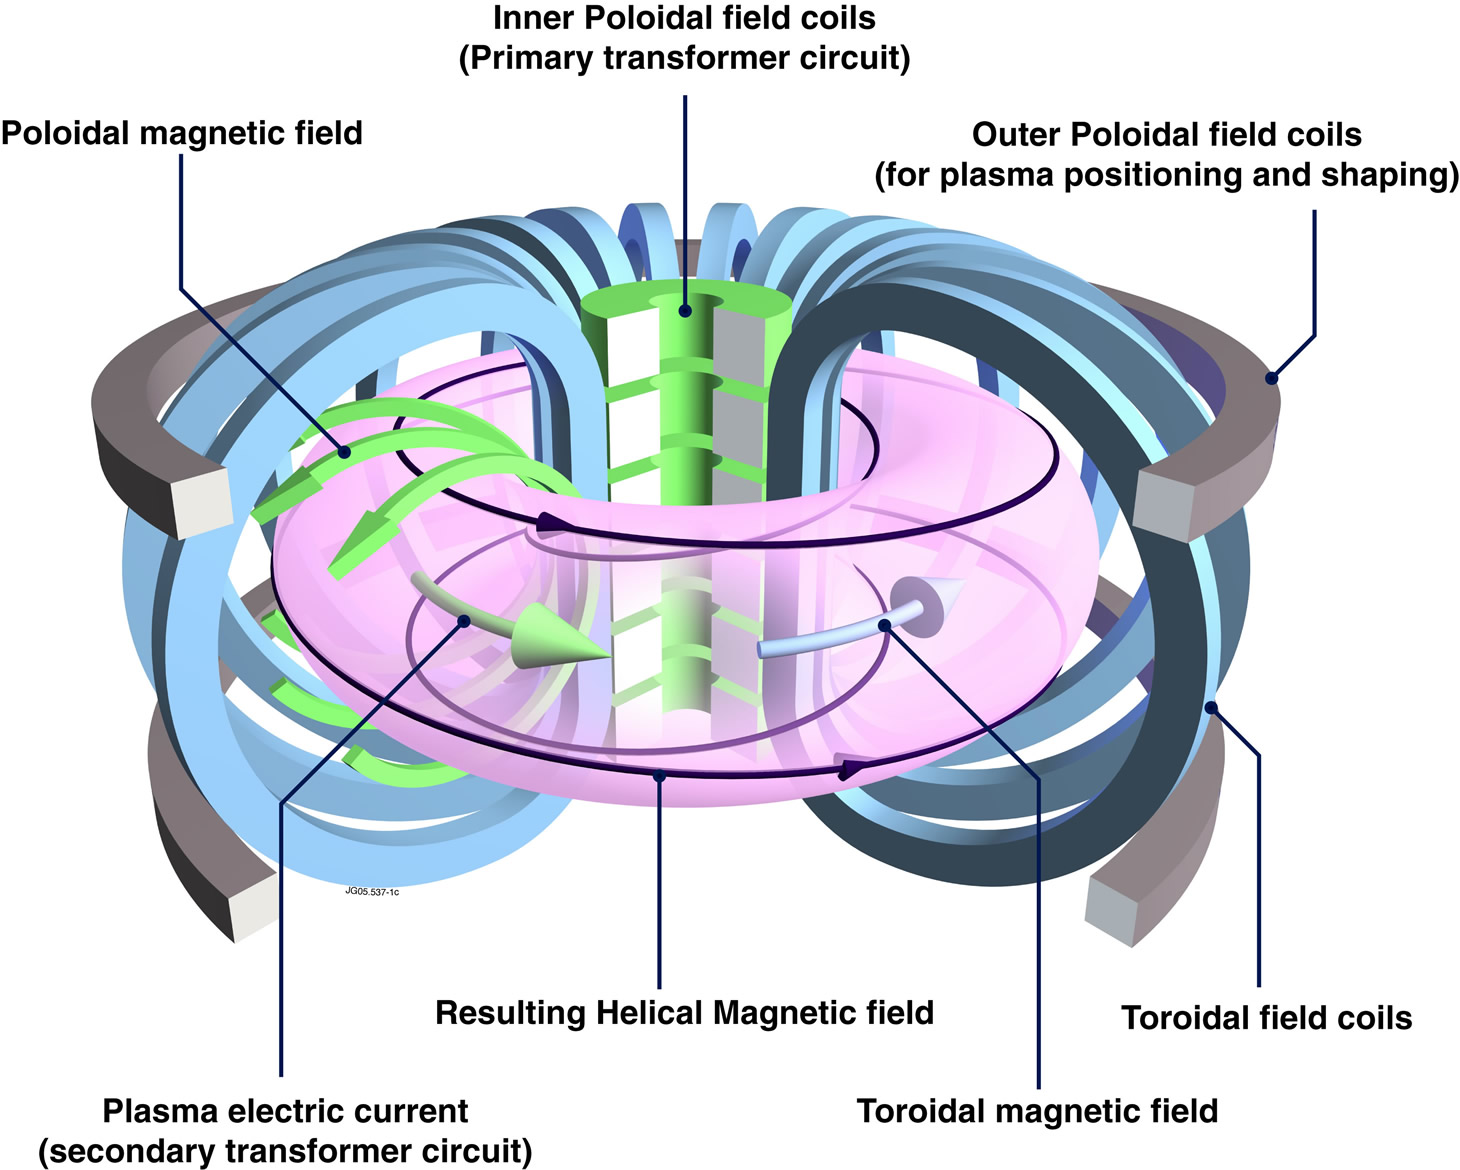
\includegraphics[height=80mm]{figures/1-tokamak.jpg}
	\caption{Schéma de principe d'un tokamak. Le terme vient du
russe (toroïdalnaïa kamera s magnitnymi katushkami : en français, chambre toroïdale avec bobines
magnétiques)~\parencite{efda}.}\label{tokamak}
\end{figure}

Le confinement de la configuration tokamak repose sur la rapidité du transport
parallèle par rapport aux processus de transport transverses
\end{refsection}
